% !TEX encoding = UTF-8 Unicode
\documentclass[a4paper]{article}

\usepackage[utf8]{inputenc}
\usepackage[T1]{fontenc}
\usepackage[slovene]{babel}
\usepackage{erk}
\usepackage{times}
\usepackage{graphicx}
\usepackage[top=22.5mm, bottom=22.5mm, left=22.5mm, right=22.5mm]{geometry}
\usepackage{array, booktabs}
\usepackage{amsmath}
\usepackage{url}

\graphicspath{{figures/}}
\def\footnotemark{}
\setlength{\emergencystretch}{2em}

\begin{document}
\sloppy

\title{Rehabilitacijski robot s prilagodljivo CMP pomočjo}

\author{Domen Brčar, Jakob Čehovin}

\affiliation{Fakulteta za elektrotehniko, Univerza v Ljubljani, Tržaška cesta 25, 1000 Ljubljana}

\email{E-mail: domen.brcar@student.uni-lj.si, jakob.cehovin@student.uni-lj.si}

\maketitle

\begin{abstract}{Povzetek}
Članek opisuje laboratorijski rehabilitacijski sistem za zgornjo okončino z
robotom Franka Emika Panda. Terapevtski gibi so zajeti z ročnim vodenjem robota
in zapisani z dinamičnimi gibalnimi primitivami (DMP), prilagodljiva robotska
pomoč pa je podana s kompenzacijskimi navorni profili CMP. Sistem loči
kinematični zapis poti od dinamičnega prispevka pomoči, zato lahko isti gib
izvede z različnimi stopnjami sodelovanja uporabnika. Za nastavitev je bil
uporabljen uporabniški vmesnik s parametrom sposobnosti od 0 do 100, kjer nižja
vrednost pomeni več dodane CMP pomoči, višja vrednost pa več samostojnega
gibanja uporabnika. Razvoj CMP pomoči je potekal postopno: najprej na
enostavnejši nalogi z dodatno utežjo, nato pri fizični interakciji z roko in
nazadnje pri rehabilitacijski vaji s tremi žogicami oziroma tremi ciljnimi
točkami. Končni sistem vključuje 3D natisnjeno držalo za roko, DMP reprodukcijo
demonstriranih gibov, skalirano CMP navorno pomoč in ponovljivo nalogo
doseganja nad delovno površino.
\end{abstract}

\section{Uvod}

Robotska rehabilitacija zgornje okončine omogoča ponovljivo izvajanje
terapevtskih nalog, merjenje poteka gibanja in nadzorovano fizično interakcijo
med uporabnikom in robotom. Pri rehabilitaciji po nevroloških poškodbah je
pomembno, da uporabnik pri nalogi aktivno sodeluje, robot pa mu pomaga v meri,
ki podpira varno, tekočo in ponovljivo izvedbo. Pregledi področja poročajo, da
lahko elektromehanski in robotski sistemi izboljšajo funkcijo roke, mišično moč
in aktivnosti vsakdanjega življenja, pri čemer so učinki povezani z zasnovo
terapije, intenzivnostjo vadbe in stopnjo uporabnikovega sodelovanja
\cite{mehrholz2018cochrane}. Že zgodnja dela s področja robot-aided
neurorehabilitation zato poudarjajo ponovljivost, merljivost in možnost
interaktivnega vodenja kot ključne prednosti robotske vadbe
\cite{krebs1998robot}.

Pri vodenju rehabilitacijskega robota ni dovolj, da manipulator sledi samo
geometrijski poti. Sistem mora biti hkrati stabilen, dovolj podajen za fizično
interakcijo in prilagodljiv različnim sposobnostim uporabnika. Zato se v
rehabilitacijski robotiki pogosto uporabljajo pristopi, povezani z impedančnim
vodenjem, kjer robot ni obravnavan le kot sledilnik položaja, temveč kot
mehanski sistem z določeno togostjo, dušenjem in interakcijskim odzivom
\cite{hogan1985impedance}. Takšna zasnova je posebej primerna za naloge, pri
katerih uporabnik vodi ali premika roko v stiku z robotom.

V predstavljenem sistemu je terapevtski gib opisan z dinamičnimi gibalnimi
primitivami. DMP so primerni za učenje iz demonstracij, ker iz izmerjene
trajektorije zgradijo stabilen dinamični model, ki ga je mogoče gladko
reproducirati in časovno skalirati \cite{schaal2006dmp,ijspeert2013dmp}. V
robotiki se uporabljajo kot standardno orodje za zapis motoričnih spretnosti,
generalizacijo gibov in delo v kontaktu z okoljem \cite{saveriano2023dmp}. Za
dodatno pomoč pri izvedbi je uporabljen koncept kompenzacijskih navornih
profilov CMP, ki poleg kinematične poti modelirajo še dinamični prispevek naloge
\cite{denisa2016cmp,petric2018cmp}. Cilj dela je izvedba celovite laboratorijske
demonstracije, ki združuje DMP učenje gibov, CMP pomoč, nastavljivo stopnjo
sodelovanja uporabnika in mehanski vmesnik za razgibavanje roke.

\section{Metode}

\subsection{DMP zapis giba}

Gibi so obravnavani v sklepnem prostoru robota Panda. Vsak od sedmih sklepov je
opisan kot časovni signal položaja in hitrosti, demonstracija pa določa začetno
lego, končno lego in obliko gibanja. Diskretni DMP za posamezen sklep uporablja
kanonično fazno spremenljivko $x$, ki monotono pada od začetka proti koncu giba:
\begin{equation}
    \tau \dot{x} = -a_x x ,
    \label{eq:canonical}
\end{equation}
kjer $\tau$ označuje trajanje giba. Transformacijski sistem za sklepni položaj
$y$ je podan z
\begin{equation}
    \tau \dot{z} = a_z \left(b_z (g-y) - z \right) + f(x),
    \qquad
    \tau \dot{y} = z ,
    \label{eq:transform}
\end{equation}
kjer je $g$ ciljna lega sklepa. Pri izbiri $b_z=a_z/4$ je osnovni del sistema
kritično dušen in zato stabilno konvergira proti cilju. Obliko demonstriranega
giba določa nelinearni člen
\begin{align}
    f(x) &=
    x\frac{\sum_{i=1}^{N} \psi_i(x) w_i}
         {\sum_{i=1}^{N} \psi_i(x)}, \nonumber\\
    \psi_i(x) &= \exp\left(-\frac{(x-c_i)^2}{2\sigma_i}\right),
    \label{eq:forcing}
\end{align}
kjer so $\psi_i$ lokalne bazne funkcije, $w_i$ pa uteži, določene iz
demonstracije z metodo najmanjših kvadratov.

V predstavljenem sistemu se DMP identificira ločeno za vse sklepe. Iz ročno
zajete demonstracije dobimo zaporedje sklepnih položajev $q(t)$ in hitrosti
$\dot{q}(t)$, iz katerih se naučijo uteži DMP modela. Rezultat učenja ni surov
posnetek, temveč gladka referenca $q_\mathrm{ref}(t)$ in
$\dot{q}_\mathrm{ref}(t)$, ki jo lahko robot ponovi pri avtomatski izvedbi.
Takšen zapis je primeren za rehabilitacijsko nalogo, ker omogoča ponovljivo
izvedbo istega terapevtskega giba in hkrati ohranja obliko demonstracije, ki jo
je določil operater z ročnim vodenjem.

\subsection{CMP pomoč}

DMP določa kinematični potek gibanja, ne določa pa neposredno, koliko dodatnega
navora naj robot prispeva med fizično interakcijo. Pri rehabilitaciji je ta
razlika pomembna: robot sledi terapevtski poti, hkrati pa uporabniku nudi mehko
pomoč, ki se lahko spreminja glede na njegovo trenutno sposobnost. CMP pristop
zato obravnava navorni signal kot dodatno primitivo, naučeno iz meritev pri
izvedbi naloge. Sorodna dela kažejo, da so takšni interakcijski signali posebej
pomembni pri gibih v kontaktu z okoljem ali človekom \cite{gams2014coupling}.

Postopek učenja CMP poteka v dveh korakih. Najprej robot avtomatsko izvede DMP
referenco, med izvedbo pa se merijo sklepni položaji, hitrosti in navori. Nato
se izmerjeni navori zapišejo z enakim principom kot sklepni položaji, kar poda
gladek profil $\tau_\mathrm{CMP}(t)$. Ta profil ni glavna trajektorija, ampak
feedforward pomoč, ki se pri rehabilitacijski izvedbi doda ukazu robota:
\begin{equation}
    \tau_d(t) =
    r(t)\, k_\mathrm{CMP}\,\alpha\,\tau_\mathrm{CMP}(t).
    \label{eq:tauadd}
\end{equation}
Faktor $r(t)$ predstavlja rampo ob začetku in koncu giba, s katero se zagotovi
zvezen vklop dodatnega navora. Parameter $\alpha$ je določen iz ocene sposobnosti
uporabnika $S$:
\begin{equation}
    \alpha=\frac{100-S}{100}, \qquad S\in[0,100].
    \label{eq:alpha}
\end{equation}
Nizka vrednost $S$ pomeni, da sistem doda več CMP pomoči. Visoka vrednost $S$
pomeni, da uporabnik opravi več gibanja sam, CMP pomoč pa je manjša. Pred
pošiljanjem robotu se dodatni navor omeji:
\begin{equation}
    \tau_d(t) = \mathrm{clip}\left(\tau_d(t),
    -\tau_\mathrm{lim},\tau_\mathrm{lim}\right).
    \label{eq:clip}
\end{equation}

Za nalogo z žogico so bili CMP profili naučeni ločeno za gib proti cilju in za
povratni gib. To je pomembno, ker povratna smer ni nujno dinamično enaka
časovno obrnjeni smeri naprej. Gravitacijski prispevek, začetna konfiguracija,
kontakt z uporabnikom in smer premika lahko povzročijo drugačen navorni profil.
Ločeni profili omogočajo bolj tekoče prehode in bolj stabilno zaporedno izvedbo
nalog.

\subsection{Postopen razvoj CMP pomoči}

Razvoj CMP pomoči je bil izveden postopno. Prvi preizkusi so bili izvedeni na
enostavnejši nalogi z dodatno utežjo, kjer je bilo mogoče jasno opazovati vpliv
dodatne obremenitve na gibanje. Pri tem so se spremljali trajanje demonstracije,
sklepne hitrosti in potreben navorni prispevek. Takšna naloga je bila uporabna
kot osnovni laboratorijski korak, saj je obremenitev na pregleden način povečala
dinamični del naloge in s tem omogočila razvoj postopka za učenje CMP profilov.
Pilotna primerjava z dodatno obremenitvijo je prikazana na
sliki~\ref{fig:obremenitev}.

\begin{figure}[!htb]
    \begin{center}
        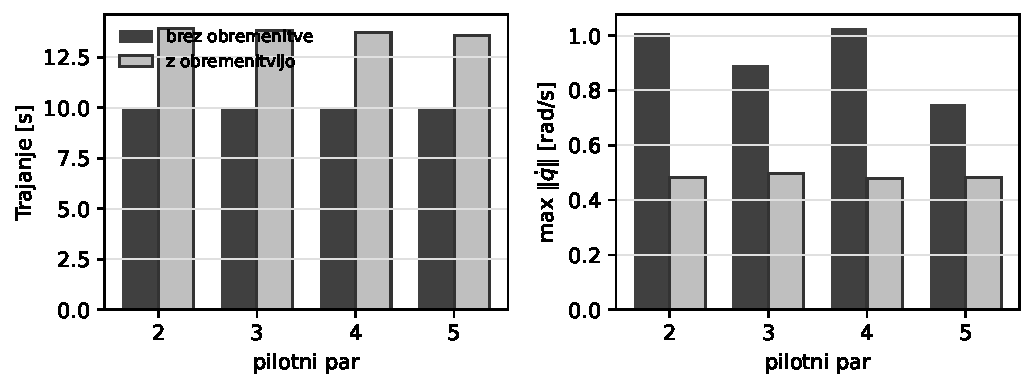
\includegraphics[width=\columnwidth]{obremenitev_pilot.pdf}
        \caption{Pilotna primerjava trajanja in največje norme sklepnih hitrosti pri demonstracijah brez dodatne obremenitve in z njo.}
        \label{fig:obremenitev}
    \end{center}
\end{figure}

Po osnovni obremenitveni nalogi je bil pristop preverjen še pri gibu, kjer
uporabnik oziroma operater z roko neposredno sodeluje z robotom. Ta korak je
dodal fizično interakcijo med človekom in manipulatorjem ter približal delovanje
sistema rehabilitacijskemu scenariju. Na osnovi obeh korakov je bila pripravljena
končna vaja, pri kateri pacient nad delovno površino dosega tri žogice oziroma
tri ciljne točke. Razvoj je tako potekal od osnovne obremenitve, prek interakcije
z roko, do bolj smiselne rehabilitacijske naloge s tremi cilji.

\subsection{Uporabniški vmesnik za nastavitev pomoči}

Za uporabo sistema je bil pripravljen uporabniški vmesnik, ki omogoča nastavitev
stopnje pomoči od 0 do 100. Parameter predstavlja sposobnost oziroma samostojnost
uporabnika pri izvedbi naloge. Pri nizki vrednosti sistem doda več CMP pomoči,
kar je primerno za uporabnika, ki pri gibu potrebuje izrazitejšo podporo. Pri
visoki vrednosti uporabnik opravi večji del gibanja sam, CMP pomoč pa se zmanjša.
Takšen vmesnik omogoča enostavno prilagajanje vadbe različnim uporabnikom ali
različnim fazam rehabilitacije, ne da bi bilo treba spreminjati naučene DMP
trajektorije.

\section{Programsko in eksperimentalno okolje}

\subsection{Programsko okolje}

Za programsko izvedbo je bila uporabljena interna knjižnica IJS, ki omogoča
poenoteno delo z robotskimi ukazi, zajemom podatkov in komunikacijo prek
robotskega vmesnika oziroma ROS okolja. Programska zasnova je bila razdeljena na
zajem demonstracij, učenje DMP modelov, učenje CMP profilov in končno
rehabilitacijsko izvedbo. Takšna delitev omogoča, da se posamezni deli sistema
preverjajo ločeno, nato pa se združijo v celoten rehabilitacijski cikel.

\subsection{Eksperimentalni sistem}

Eksperimentalni sistem temelji na sedemosnem robotu Franka Emika Panda z
robotskim prijemalom. Robot je nameščen ob delovni površini, na kateri so
označene ciljne točke za nalogo z žogicami. Postavitev omogoča demonstracijo
gibov, avtomatsko reprodukcijo naučenih trajektorij in fizično interakcijo z
uporabnikom. Fotografija postavitve je prikazana na sliki~\ref{fig:postavitev}.

\begin{figure}[!htb]
    \begin{center}
        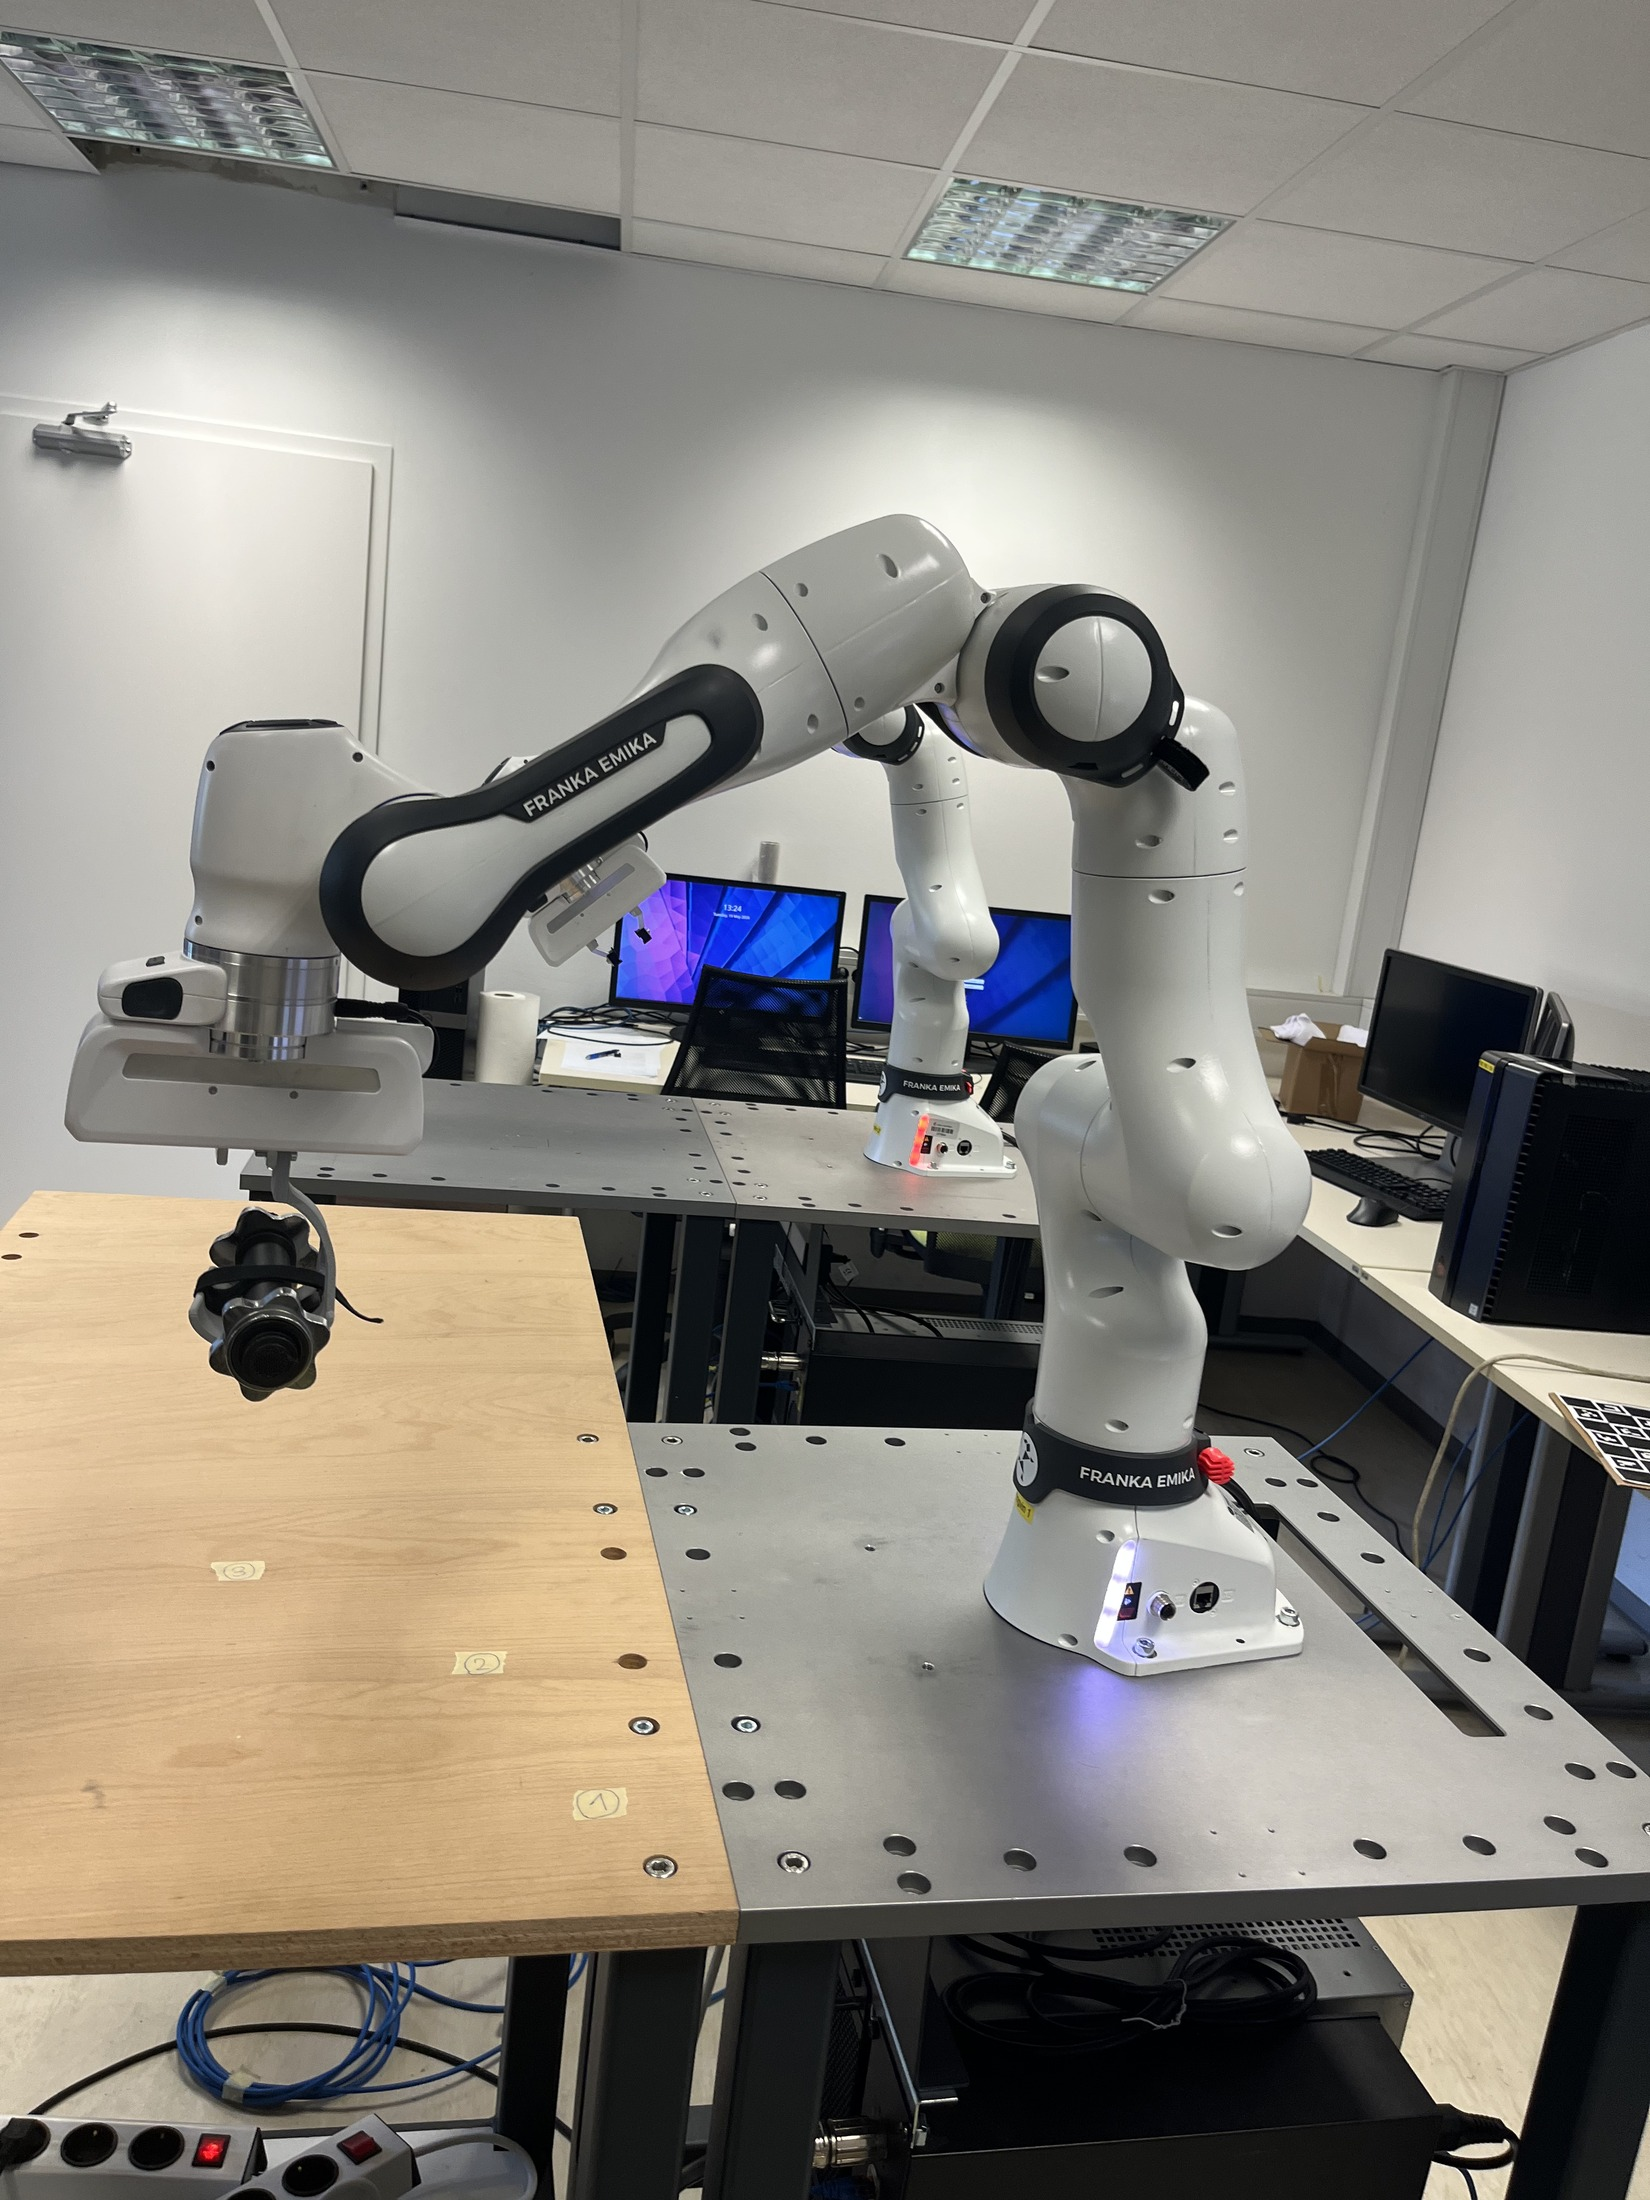
\includegraphics[width=\columnwidth]{robot_02.jpg}
        \caption{Eksperimentalna postavitev z robotom Panda, delovno površino in označenimi ciljnimi točkami.}
        \label{fig:postavitev}
    \end{center}
\end{figure}

Postopek priprave je sestavljen iz več zaporednih korakov. Najprej se robot
postavi v začetno lego, ki služi kot referenca za nadaljnje gibe. Nato se posname
osnovni premik, ki pripravi roko na izvajanje naloge, in tri trajektorije naloge
z žogico. Iz vsake demonstracije se identificira DMP model, ki poda gladko
sklepno referenco. V naslednjem koraku robot te reference izvede avtomatsko, pri
čemer se merijo navori in se iz njih naučijo CMP profili. Končna
rehabilitacijska izvedba nato združi DMP referenco, skaliran CMP navor in
stabilno držanje lege med posameznimi prehodi.

\subsection{3D natisnjeno držalo za roko}

Pomemben del sistema je mehanski vmesnik med uporabnikom in robotom. Držalo za
roko je bilo modelirano v programu Fusion 360 in izdelano s 3D tiskanjem. Oblika
je prilagojena roki, spodnji zaobljeni del pa omogoča udobnejšo oporo med
vodenjem nad delovno površino. Pritrdilne odprtine omogočajo mehansko povezavo z
robotom oziroma nastavitev položaja držala. Namen držala je varnejši, bolj
ponovljiv in udoben stik med pacientom in robotom.

Mehanski vmesnik je pomemben del sistema, saj neposredno vpliva na udobje
uporabnika, ponovljivost prijema in varnost fizične interakcije. Držalo omogoča
razgibavanje roke nad površino in vodenje proti ciljem, pri tem pa podpira
počasne, kontrolirane in ponovljive gibe. Uporabljeno držalo in stik roke z
robotom sta prikazana na sliki~\ref{fig:drzalo_roka}.

\begin{figure}[!htb]
    \begin{center}
        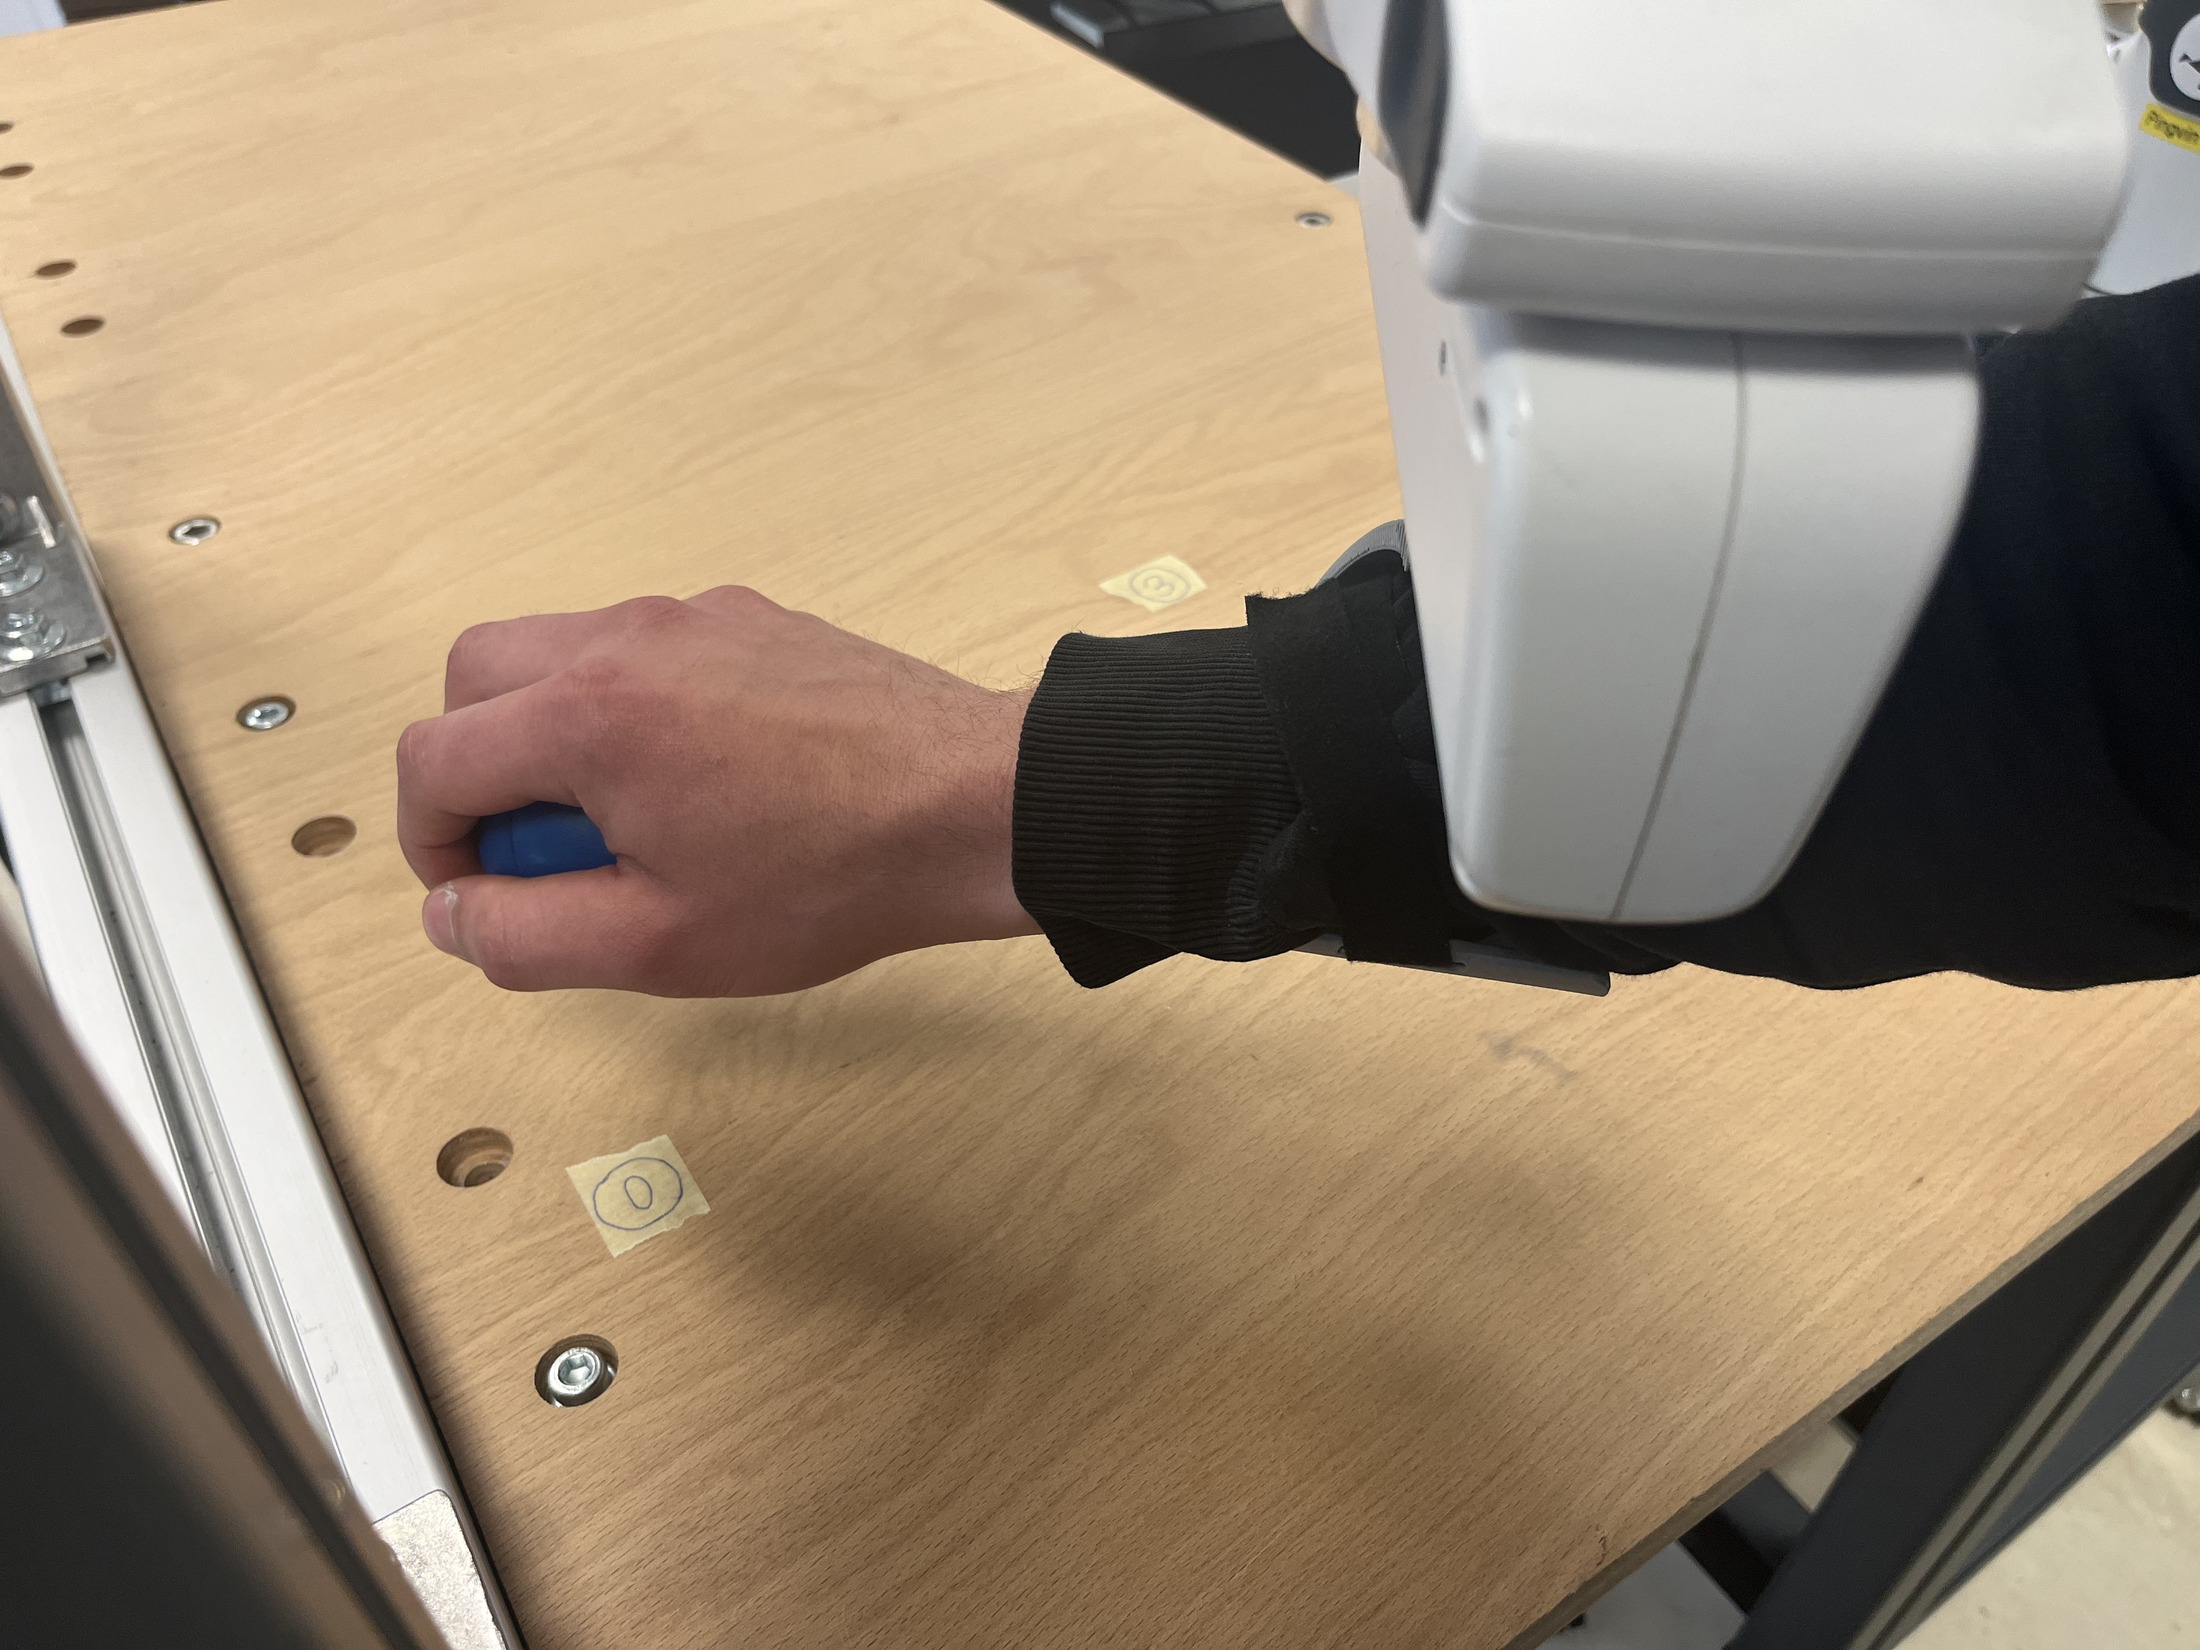
\includegraphics[width=0.85\columnwidth]{robot_04.jpg}
        \caption{3D natisnjeno držalo za roko med vodenjem uporabnikove roke nad delovno površino.}
        \label{fig:drzalo_roka}
    \end{center}
\end{figure}

\subsection{Končna rehabilitacijska naloga}

Končna naloga je zasnovana kot rehabilitacijska vaja zgornje okončine. Pacient
drži oziroma uporablja 3D natisnjeno držalo za roko, robot pa vodi oziroma pomaga
pri razgibavanju nad delovno površino. Cilj je premikanje proti trem žogicam
oziroma trem ciljnim točkam. Gibi so počasni, kontrolirani in ponovljivi, zato
je naloga primerna za vadbo doseganja, koordinacije in kontroliranega premikanja
zgornje okončine.

Med izvedbo robot po koncu posamezne trajektorije aktivno drži doseženo lego,
naslednja trajektorija pa prevzame vodenje iz stabilne konfiguracije. Takšno
obnašanje je pomembno pri delu z zgornjo okončino, saj omogoča mirne prehode med
posameznimi cilji. Glavna eksperimentalna slika naloge z doseganjem žogice je
prikazana na sliki~\ref{fig:naloga_zogica}.

\begin{figure}[!htb]
    \begin{center}
        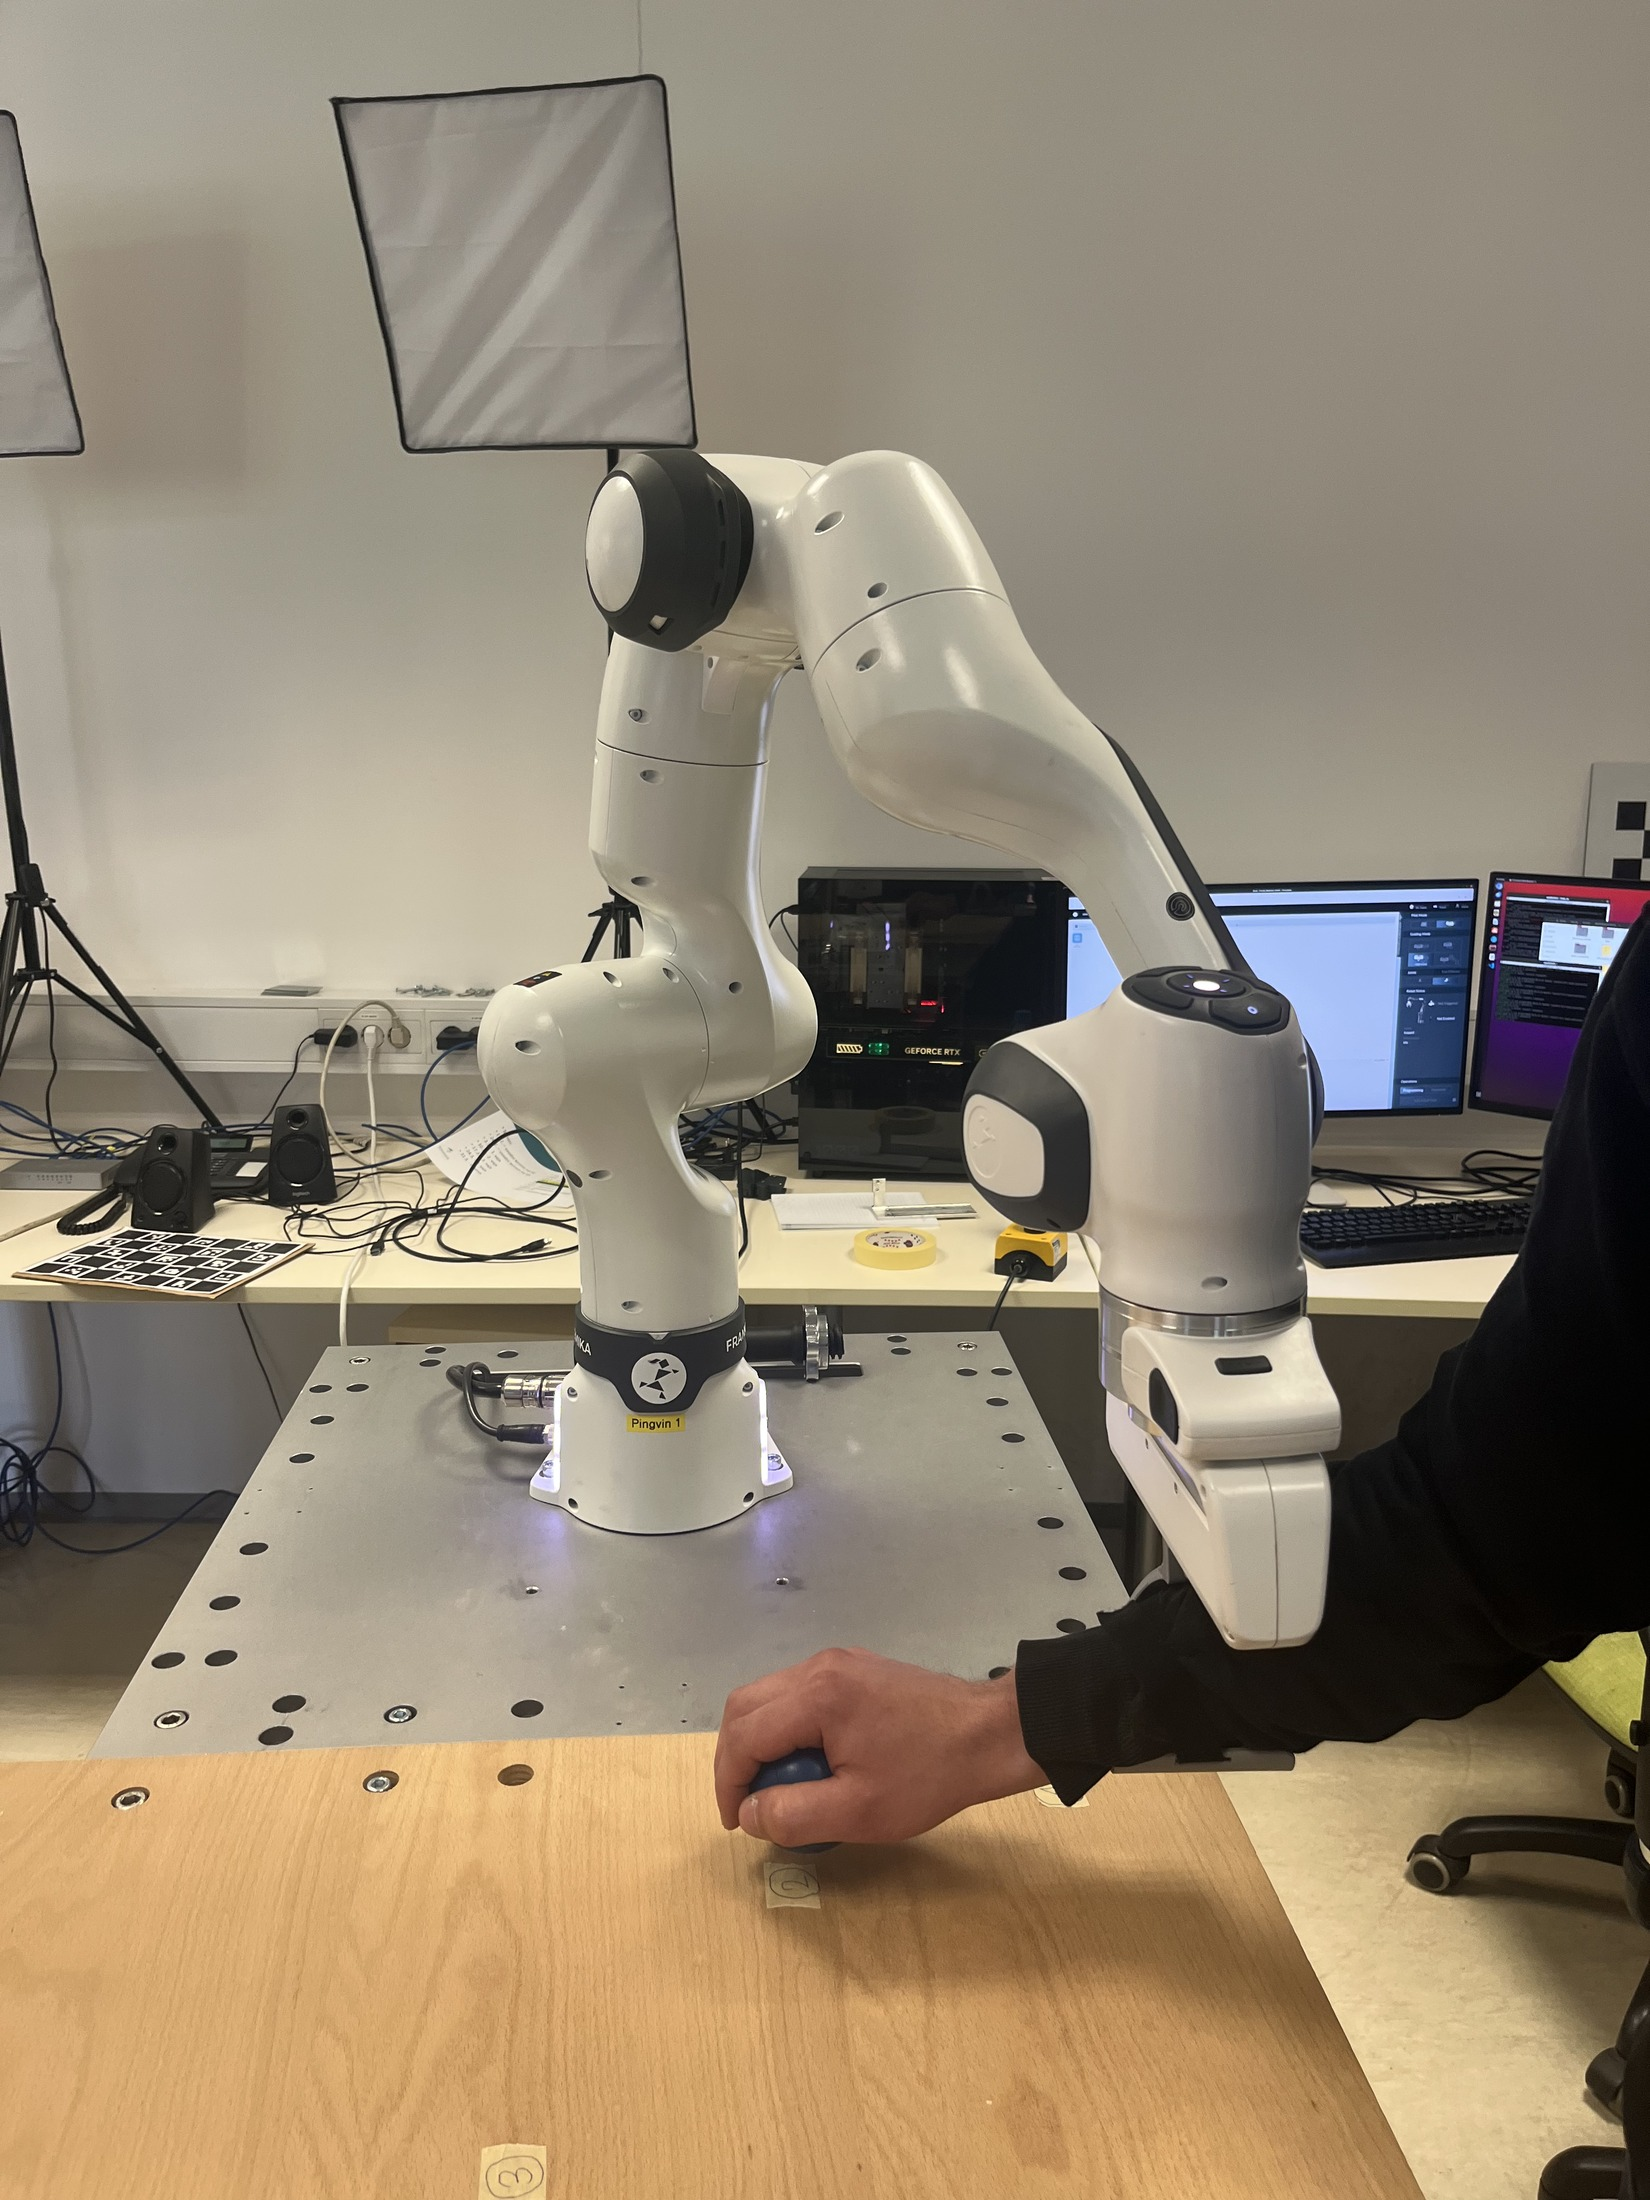
\includegraphics[width=\columnwidth]{robot_05.jpg}
        \caption{Rehabilitacijska naloga z doseganjem žogice nad delovno površino.}
        \label{fig:naloga_zogica}
    \end{center}
\end{figure}

\section{Podatki in rezultati}

Za glavni nabor rezultatov so bile zajete štiri demonstracije: osnovni premik
ter tri trajektorije naloge z žogico. Vsi signali so zapisani v sklepnem
prostoru sedemosnega robota in zajeti s frekvenco 100 Hz. Povzetek demonstracij
je podan v tabeli~\ref{tab:trajektorije}.

\begin{table}[htbp]
    \centering
    \caption{Povzetek uporabljenih demonstracij}
    \label{tab:trajektorije}
    \begin{tabular}{lccc}
        \toprule
        Gib & Vzorci & Trajanje [s] & Sklepi \\
        \midrule
        Osnovni premik & 599 & 5.98 & 7 \\
        Žogica 1 & 804 & 8.03 & 7 \\
        Žogica 2 & 610 & 6.09 & 7 \\
        Žogica 3 & 585 & 5.84 & 7 \\
        \bottomrule
    \end{tabular}
\end{table}

Demonstracije so počasne in primerne za rehabilitacijsko izvedbo. Najdaljša je
prva trajektorija naloge z žogico, ki traja približno 8 s, ostale pa trajajo med
5.8 s in 6.1 s. Takšna trajanja so skladna z nalogo, kjer je poudarek na vodeni,
nadzorovani izvedbi in ne na hitrem premiku. Sklepni poteki na
sliki~\ref{fig:sklepi} prikazujejo, da so demonstrirani gibi zvezni in
porazdeljeni po več sklepih. To je ugodno pri sedemosnem redundantnem
manipulatorju, saj se naloga izvaja kot koordinirano premikanje roke po delovni
površini.

\begin{figure}[!htb]
    \begin{center}
        
\includegraphics[width=\columnwidth]{trajektorije_sklepi.pdf}
        \caption{Sklepni poteki osnovnega premika in treh trajektorij naloge z žogico.}
        \label{fig:sklepi}
    \end{center}
\end{figure}

\subsection{CMP rezultati}

Naučeni CMP profili so povzeti na sliki~\ref{fig:cmp}. Prikazana je norma
kompenzacijskega navornega profila pred skaliranjem s parametrom sposobnosti.
Profili za nalogo z žogico imajo primerljive velikostne rede, osnovni premik pa
predstavlja začetni del zaporedja. Pri dejanski rehabilitacijski izvedbi se ti
signali skalirajo z uporabniško nastavitvijo, zvezno vklopijo z rampo in omejijo
z izbrano navorno mejo.

\begin{figure}[!htb]
    \begin{center}
        
\includegraphics[width=\columnwidth]{cmp_norme.pdf}
        \caption{Norma naučenih CMP navornih profilov za osnovni premik in nalogo z žogico.}
        \label{fig:cmp}
    \end{center}
\end{figure}

Primerjava smeri naprej in povratne smeri je prikazana na
sliki~\ref{fig:cmp_smeri}. Čeprav sta trajektoriji geometrijsko povezani, se
navorni profili med smerema razlikujejo. Ločeno učenje smeri naprej in nazaj je
zato smiselno za zaporedno nalogo s tremi cilji, ker omogoča, da je pomoč
prilagojena dejanskemu dinamičnemu poteku posameznega giba.

\begin{figure}[!htb]
    \begin{center}
        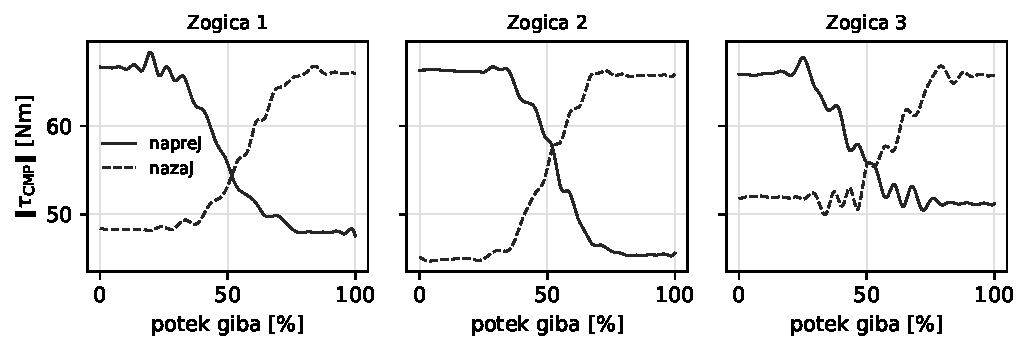
\includegraphics[width=\columnwidth]{cmp_smeri.pdf}
        \caption{Primerjava norme CMP profilov za smer naprej in povratno smer pri treh gibih z žogico.}
        \label{fig:cmp_smeri}
    \end{center}
\end{figure}

\section{Razprava}

Rezultati kažejo, da je mogoče iz ročno vodenih demonstracij pripraviti
ponovljive DMP reference in zanje naučiti CMP navorne profile. Glavna prednost
takšne zasnove je ločitev med potjo in pomočjo. DMP določa, kam in kako naj se
roka premika, CMP pa določa, koliko dodatnega navora naj robot prispeva pri
izvedbi. Zato isti terapevtski gib ni vezan na eno samo stopnjo pomoči, temveč
ga je mogoče prilagoditi uporabniku z nastavitvijo parametra sposobnosti.

Postopen razvoj od naloge z dodatno utežjo do interakcije z roko in končne
naloge z žogicami je bil pomemben za pregledno gradnjo sistema. Naloga z utežjo
je omogočila opazovanje vpliva obremenitve na trajanje, hitrosti in navorni
prispevek. Interakcija z roko je dodala fizični stik med robotom in uporabnikom,
končna naloga s tremi cilji pa je povezala naučene metode v rehabilitacijsko
smiselno vajo. Tak razvojni potek je dobra osnova za nadaljnje razširitve, saj
vsak korak preverja drug del celotnega sistema.

Nastavljiva pomoč prek uporabniškega vmesnika je pomembna za praktično uporabo.
Parameter od 0 do 100 omogoča hitro spremembo stopnje pomoči brez ponovnega
učenja DMP trajektorij ali CMP profilov. Sistem se tako lahko prilagodi
različnim uporabnikom, različnim dnevnim stanjem uporabnika ali postopnemu
napredku med rehabilitacijo. Pri nižji vrednosti parameter poveča robotsko
podporo, pri višji vrednosti pa spodbuja več samostojnega gibanja.

Mehanski vmesnik v obliki 3D natisnjenega držala dopolnjuje programski del
sistema. Držalo vpliva na udobje, ponovljivost stika in občutek varnosti med
fizično interakcijo. V laboratorijski izvedbi zato nima le mehanske vloge,
temveč povezuje robotsko vodenje s pacientovo roko in omogoča kontrolirano
razgibavanje nad delovno površino. Za nadaljnje delo je smiselno sistem
vrednotiti pri več ponovitvah in različnih nastavitvah pomoči ter spremljati
napako sledenja, dodani CMP navor, uspešnost doseganja ciljev in uporabnikov
občutek napora.

\section{Zaključek}

Predstavljen je bil celovit laboratorijski sistem za robotsko podprto
rehabilitacijsko vajo zgornje okončine. Sistem združuje demonstracijo gibov,
DMP reprodukcijo, CMP navorno pomoč, nastavljivo stopnjo pomoči prek
uporabniškega vmesnika, 3D natisnjen mehanski vmesnik za roko in nalogo s tremi
cilji oziroma žogicami. Končna izvedba omogoča počasno, kontrolirano in
ponovljivo razgibavanje roke nad delovno površino, pri čemer lahko robot stopnjo
pomoči prilagodi izbrani sposobnosti uporabnika. Takšna zasnova predstavlja
uporabno osnovo za nadaljnje nadgradnje robotsko podprte rehabilitacije, zlasti
za podrobnejše vrednotenje prilagodljive pomoči in mehanske ergonomije držala.

\small
\bibliographystyle{ieeetr}
\bibliography{references}

\end{document}
